\section{Les Résonances de Moyen Mouvement (MMR)}
\subsection{Définition}\index{résonance!de Moyen Mouvement}\index{Mean Motion Resonance|see{résonance}}
Les \gras[resonance@résonance]{résonances de moyen mouvement} sont des configurations orbitales particulières de deux planètes dans lesquelles il existe un lien entre les périodes orbitales des planètes. Exemple, si deux planètes sont en résonance $3:2$, ça signifie que la planète interne effectuera 3 orbites pendant que la planète externe en effectuera 2.

Ces configurations particulières confèrent une stabilité accrue aux planètes. Plus la résonance est forte et plus il sera difficile pour les planètes d'en sortir.

\bigskip

On met généralement une résonance sous la forme $(p+q):p$ où $p$ et $q$ sont des entiers. Cette forme permet de mettre en évidence un des paramètres qui permet de rendre compte de la force de la résonance. En effet, plus $q$ est petit et plus la résonance est forte. Ainsi, les résonances d'ordre 1 ($q=1$) sont les plus fortes. On dit que $q$ est l'ordre de la résonance (plus l'ordre est petit et plus la résonance est forte). De même, $p$ est le degré de la résonance.

\begin{attention}
Mais ce n'est pas le seul paramètre à prendre en compte pour évaluer la force d'une résonance et je suis bien incapable de tous les décrire.
\end{attention}

Pour une résonance $(p+q):p$ on définit un certain nombre d'angles $\theta_i$ dits \gras[angle de résonance]{angles de résonance} de la forme :
\begin{align}
\theta_{i+1} &=(p+q)\lambda_2 -p\lambda_1 - \left[i\varpi_{1} + (q-i)\varpi_2\right]
\end{align}
avec $i$ allant de $0$ à $q$ ; où $\lambda$ sont les longitudes moyennes, $\varpi$ les longitudes du péricentre et les indices $1$ et $2$ se réfèrent respectivement à la planète interne et externe. Pour une résonance $(p+q):p$ on a donc $q+1$ angles de résonance.

Les angles de résonances mesurent l'angle entre les deux planètes au point de conjonction. Si un seul de ces angles est en libration (oscillation autour d'une valeur moyenne) au lieu de circuler librement de $0$ à $2\pi$ alors on dit que les planètes sont en résonances. Le nombre d'angles en libration permettra aussi d'avoir une idée de la force de la résonance.

\begin{exemple}
Soit une résonance $7:2$, les angles de résonances sont :
\begin{align*}
\theta_1 &= 7 \lambda_2 -2\lambda_1 - 5 \varpi_1\\
\theta_2 &= 7 \lambda_2 -2\lambda_1 - \left( 4 \varpi_1 + 1\varpi_2 \right)\\
\theta_3 &= 7 \lambda_2 -2\lambda_1 - \left( 3 \varpi_1 + 2\varpi_2 \right)\\
\theta_4 &= 7 \lambda_2 -2\lambda_1 - \left( 2 \varpi_1 + 3\varpi_2 \right)\\
\theta_5 &= 7 \lambda_2 -2\lambda_1 - \left( 1 \varpi_1 + 4\varpi_2 \right)\\
\theta_6 &= 7 \lambda_2 -2\lambda_1 - 5 \varpi_2
\end{align*}
\end{exemple}

\begin{remarque}
Les \gras[kirkwood@Kirkwood!lacunes de]{lacunes de Kirkwood} font elles aussi intervenir des résonances mais contrairement à ce qu'on pourrait penser, ces résonances avec Jupiter sont des zones déplétées en astéroïdes. 

La résonance imposte une valeur de $a$, mais des échanges sont possibles entre les deux corps en résonance et il est possible que par ce biais l'excentricité puisse augmenter, et ainsi dépléter la lacune de kirkwood en favorisant les collisions entre les objets en résonance et les autres qui sont dans la ceinture.
\end{remarque}


%TODO MMR : lire a thorough analysis of the dunamics involved the reader should consult (Murray & Dermott, 1999)
%TODO cité depuis chapitre 8 resonant perturbations : 
% useful reviews of the subject, particularly in the context of orbital evolution through resonance, have been given by Greenberg (1977), Peale (1986) and Malhotra (1988).
%TODO 
\subsection{Résonances et excentricité}
Cela dépend de l'ordre et du degré de la résonance, mais les perturbations gravitationnelles mutuelles de deux corps en résonance de moyen mouvement engendrent des modifications des éléments orbitaux de ces derniers. 

En particulier, l'excentricité de deux corps en résonance a tendance à varier augmenter au cours du temps \citep[eq. (8.29)]{murray2000solar}. 

Nous n'allons pas détailler ici le fonctionnement précis des résonances. Plusieurs auteurs traitent de ce sujet \citep{greenberg1977orbit, peale1986orbital, malhotra1988phd}. C'est un sujet extrêmement complexe, que je ne maitrise absolument pas dans les détails. De plus, dans le cadre de notre étude de la formation des planètes, nous sommes dans un cas un peu différent. Les résonances entre planète ont lieu dans un système dissipatif, le disque protoplanétaire, qui agit sur les éléments orbitaux, par exemple en amortissant l'excentricité et l'inclinaison des planètes.

Il est difficile de prendre pour exemple les cas N-corps classiques et essayer de les appliquer dans le disque de gaz. Dans notre cas, l'amortissement de $e$ et $I$ par le disque stabilise les résonances, empêchant les résonances normalement instables de se briser. Bien entendu, les résonances se brisent dans nos systèmes en formation, mais dans des cas beaucoup plus extrêmes, notamment quand on a une chaîne de résonance contenant plusieurs corps, tous en résonance. 

Dans de tels systèmes, on constate plusieurs tendances. 

\subsection{Effet du rapport de masse}
%phd/MMR_mass_ratio

%TODO
\subsection{Effet du nombre de corps en résonance}




%TODO 
\subsection{Stabilité et ordre des résonances}

\begin{figure}[htb]
\centering
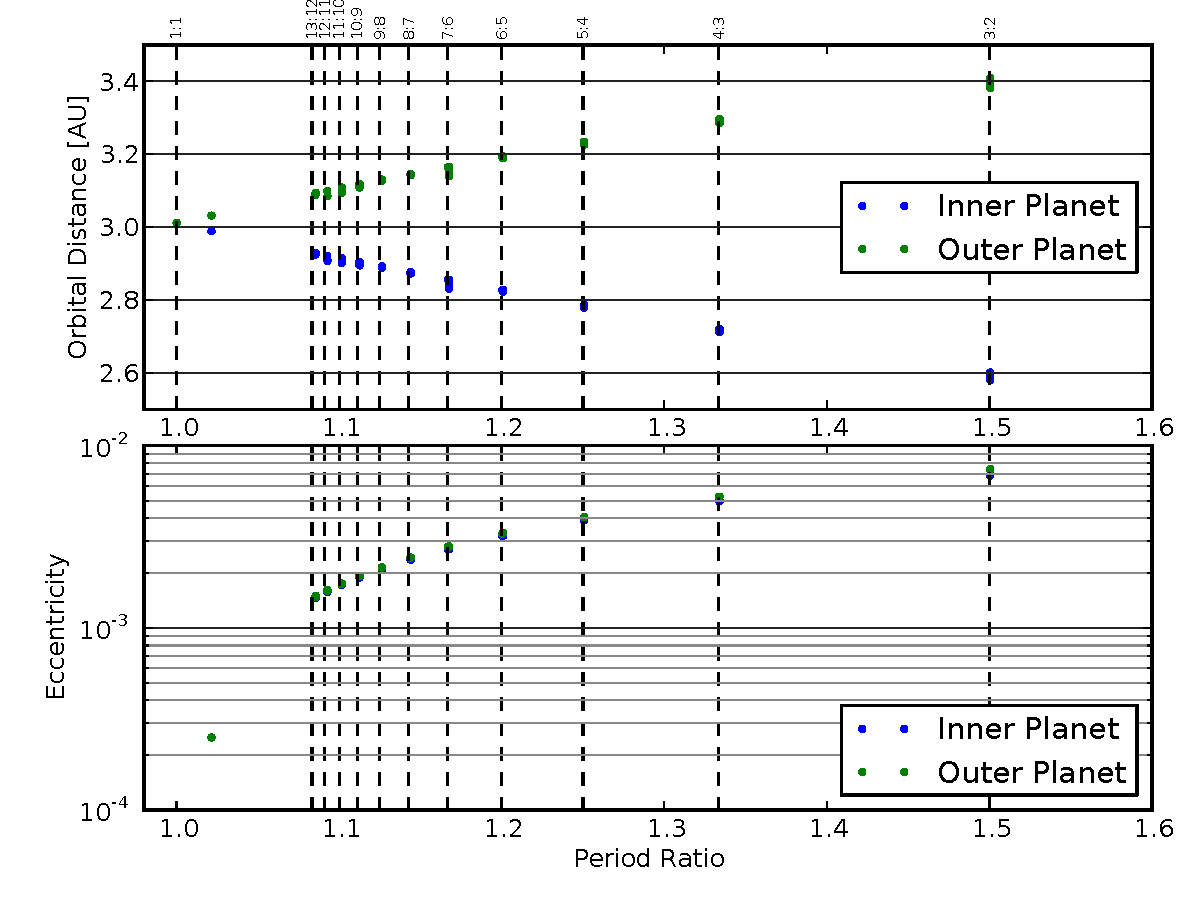
\includegraphics[width=0.75\linewidth]{figure/MMR_statistique.pdf}
\caption{Illustration des différentes résonances possibles et de l'augmentation de l'excentricité qu'elles entrainent. Chaque simulation contenait deux planètes de $1\mearth$ aléatoirement réparties entre $1$ et $10\unit{AU}$. Chaque point correspond à une planète. }\label{fig:MMR_statistique}
\end{figure}
%TODO 

\section{Les Zones de Convergence}
%TODO 
\subsection{Existence et intérêt}
%TODO 
\subsection{Les différents types}\label{sec:CZ-types}
%TODO 
\subsection{Diagrammes de couple a-m}\label{sec:migrations-maps}
%TODO parler des raisons pour lesquelles la zone de convergence dépend de la masse et de la distance parfois, avec les comparaisons des temps (dynamique, de U-turn and de diffusion)
\subsection{Résonances et Accrétions}
%TODO 